%%%%%%%%%%%%%%%%%%%%%%%%%%%%%%%%%%%%%%%%%%%%%%%%%%%%%%%%%%%%%%%%%%%%%%
% writeLaTeX Example: Academic Paper Template
%
% Source: http://www.writelatex.com
% 
% Feel free to distribute this example, but please keep the referral
% to writelatex.com
% 
%
%%%%%%%%%%%%%%%%%%%%%%%%%%%%%%%%%%%%%%%%%%%%%%%%%%%%%%%%%%%%%%%%%%%%%%
\documentclass[twocolumn,showpacs,%
  nofootinbib,aps,superscriptaddress,%
  eqsecnum,prd,notitlepage,showkeys,10pt]{revtex4-1}

\usepackage{amssymb}
\usepackage{amsmath}
\usepackage{graphicx}newline
\usepackage{dcolumn}
\usepackage{hyperref}
\usepackage{float}
\usepackage{caption}

\begin{document}

\title{Analyzing Policy Restrictions on Institutional Investors: An Agent Based Model of Atlanta, Georgia's Housing Market}
\author{Anirudh Thodupunuri}
\affiliation{ICR 2026}

\begin{abstract}

Institutional investors have emerged as a significant presence within the single-family real estate market, which has prompted a wave of legislation addressing their impact, culminating in the 21st Century ROAD to Housing Act of 2026. However, empirical evidence on investor impacts remains mixes, and comparison of specific policies is lacking. This paper develops and calibrates an agent-based model of the Atlanta, Georgia housing market to evaluate six different proposed institutional investor restriction policies: waiting periods, soft and hard ownership caps, purchase taxes, vacancy taxes, and progressive portfolio taxes. The model is calibrated to 2019 Atlanta through tract-level ACS census data, HMDA mortgage records, and Zillow price and rent indices, and runs 40 stochastic seeds per policy scenario. Results reveal a consistent outperformance of access restrictions compared to financial penalties, with the waiting period producing the largest homeownership improvement at $+3.3\%$ relative to baseline. The waiting period also simultaneously increases rental vacancy rate, avoiding the trade-off between homeownership and rental supply that is experienced by the ownership caps. Financial penalties produce negligible effects, reflecting the cushion that Atlanta's gross rental yield of $8.28\%$ provides against tax surcharges. These findings suggest that the ownership cap enacted in the ROAD act may improve homeownership at the cost of tightening rental supply, and that waiting period mechanisms, not currently included in federal legislation, should be considered as well as or instead of the existing ownership cap. 


\end{abstract}

\maketitle

\section{Introduction}

\subsection{Background}

Following the 2008 Financial Crisis, housing has exploded into one of the cardinal challenges of the modern era. The housing market is indicative and a significant driver of many economic dynamics: consumer spending, inflation, labor mobility and financial system stability. Consisting of a complex set of interactions between different sets of agents, the housing market includes but is not limited to renters, first time buyers, repeat buyers, small landlords and institutional investors. Understanding how policy interventions affect these interactions is critical to addressing the affordability crisis plaguing households across the country. \newline

When modeling these complex interactions, standard techniques are often insufficient. Dynamic stochastic general equilibrium (DSGE) models, which dominated policy analysis prior to the financial crisis, assume a perfectly rational agent at their core. Thus, by construction the models fail to capture emergent dynamics \cite{tesfatsion2006} that characterize a realistic housing market. These oversimplifications can lead policymakers astray and famously fail to predict crises such as the aforementioned financial crisis. \newline

Agent based models (ABMs) present an alternative to the traditional methods that is better suited for modeling the real estate market. Agent based models are computational simulations where individual, autonomous agents interact in an environment, following some set of rules. Because agents are independent, heterogeneity can be realized in the population to a greater extent, with agents initialized following a realistic distribution of wealth, income, and other defining fields. Moreover, non linear dynamics (booms and busts) are expressed in agent based models due to the interactions between buyers and sellers in the market. 
ABMs are also effective for testing the impacts of policies targeted at limiting sections of the population, as interventions can be applied to specific agent types and their downstream effects can be traced. \newline

\subsection{Motivation}

A growing body of work has already applied ABMs to the housing market. A foundational paper in the field, Axtell et al. (2014) \cite{axtell2014} modeled the housing bubble in Washington D.C. and found that tighter interest rate policies would have done little to prevent the bubble from forming. The primary reference for this paper, Baptista et al. (2016) (2016)\cite{baptista2016}, extended this approach to the UK housing market while incorporating a life-cycle household structure and a double auction clearing mechanism. However, existing ABM studies have focused on macroprudential policies that affect the market as a whole, rather than investor-specific restrictions that have become a dominant focus within the current housing policy in the US. \newline

Institutional investors, with regard to housing, are large entities that pool capital in order to invest in real estate on behalf of their shareholders. These investors focus on multifamily apartment complexes and single family rental homes, with institutional portfolios representing 589,000 homes or roughly $3.9\%$ of the single family rental market \cite{urbaninvestor2022}. Out of concern that these investors outcompete first-time buyer families and lead to price growth, legislators have proposed restrictions on their activity. On January 20, 2026, an executive order directed federal agencies to limit support for single family home sales to large institutional investors. In July 2026, the 21st Century ROAD to Housing act, widely considered to be one of the most significant pieces of federal housing legislation in decades, became law. This bipartisan legislation prohibits institutional investors from purchasing additional single family homes, though it includes certain exceptions (build-to-rent, for example). \newline 

However, the empirical evidence on the impacts of institutional investors carries mixed results. Some studies find meaningful price and displacement effects in areas with high investor concentration, while others argue that investors represent too small of a share of the market to have market-wide implications, and may in some cases improve housing supply by renovating distressed homes. This paper addresses the need for rigorous policy analysis, especially to find which specific restriction mechanism produces the best outcomes over many different metrics. \newline

In this paper, we develop and calibrate an agent based model of the Atlanta, Georgia housing market, one of the metro areas most affected by institutional investor activity. We use this model to evaluate distinct policies: waiting periods, ownership caps, purchase taxes, vacancy taxes, and progressive portfolio taxes. For each policy, we measure effects on three outcomes simultaneously: first time homeownership rate, rental vacancy, and housing price appreciation. Our market is calibrated to the 2019 Atlanta conditions using tract-level Census data, assessor records, HMDA mortgage data, and Zillow price and rent indices, with validation against the 2020-2023 period before policy experiments are conducted. In doing so, we answer the question \textit{Among policies aimed at restricting institutional investor activity, which maximizes first-time homeownership rates while minimizing volatility in rental vacancy rate and housing price appreciation?}\newline

The remainder of the paper proceeds as follows. Section 2 describes the model structure and agent types. Section 3 details the data sources and calibration strategy. Section 4 presents the experimental design. Section 5 reports results. Section 6 discusses the implications of these results. Section 7 concludes, and Appendix A details the equations used in the model. 





\section{Model Description}
\label{sec:examples}

\subsection{Overview}

We develop an agent-based model of the single family residential housing market in the Atlanta metropolitan area, encompassing Fulton, DeKalb, Gwinnett, Cobb, Clayton, Henry and Paulding counties. The model operates on monthly time steps, where each steps represents a calendar month. The spatial unit is the census tract, a small stable geographical region with a population of around 4000. Approximately a thousand of these tracts exist within the chosen area, each containing its own price level, rental rate, vacancy rate and investor concentration. However, as a simplification the model currently only uses one representative tract, with multi-tract modeling as a planned extension. The model is initialized to 2019 conditions using empirical data, then run forward through time as core macro level housing outcomes are tracked. \newline

Agent population evolves each period through births, deaths, and aging. New housing supply is added via a construction mechanism to maintain the house-to-household ratio. \newline

The model follows the general architecture established in the mentioned papers, Axtell et al. (2014) and Baptista et al. (2016), with modifications to reflect the US institutional investor context. The core change from these models is the distinction between institutional investors and small landlords as well as the implementation of the different investor focused policies. Mathematical specifications of the used equations are provided in Appendix A. 

\subsection{Agent Types}

The model contains six agent types. Five are decision making agents in the traditional sense, whose behavior drives the market dynamics. The final agent is a passive, state-holding agent representing the physical household stock. \newline

\textbf{First Time Buyers:}
First time buyer agents (FTBs) represent households seeking to purchase their first home, as they have previously been renting. They are distinguished from repeat buyers by their lack of existing home equity, and a stronger psychological preference for ownership (shown through the $(1+\tau)$ term in equation (5), where FTBs decide between renting and buying. FTBs accumulate savings each period from their income, subtracting rent and consumption expenditures, and enter the ownership market when their savings exceed the minimum down payment for an FHA mortgage ($3.5\%$ of target purchase price). Once they are in the market, they evaluate listings based on their constrained budget, compete against other buyers and investors, then exit back to renting if the search takes too long without a successful purchase . The primary interest of this study is the first-time buyer share of transactions. \newline

\textbf{Repeat Buyers:} Repeat buyer agents represent households purchasing a subsequent home, while already owning and living in a previous home. As mentioned before, repeat buyers have existing home equity available as a down payment, which gives them a larger budget ceiling and access to conventional mortgage terms ($20\%$ down/$80\%$ loan-to-value ratio.) When a repeat buyer purchases a new home, they simultaneously make the decision between selling their previous home or placing it on the rental market. This decision is governed by a comparison between the expected rental yield and the opportunity cost of the capital gained by selling. An adaption we make is adding a mortgage lock-in effect: when prevailing interest rates substantially exceed the rates on their existing mortgage, repeat buyers probability of selling and moving falls, reducing market liquidity. This is known as the "golden handcuffs" effect \cite{fonseca2023lockin} and is important to reproducing the transaction volume decline observed in Atlanta following the COVID-19 pandemic (2022-2023). \newline

\textbf{Small Landlords:} Small landlord agents (mom-and-pop landlords) represent individual investors owning between two and ten residential units. Their strategy is primarily income focused, placing greater weight on rental yield (immediate, regular cash flow) rather than capital appreciation (long term wealth creation). Small landlords set rents with downward stickiness: at each lease renewal, they only update rent toward market rate with $60\%$ probability, and they never reduce rents while a tenant is in place. This adaption, grounded in survey evidence on individual landlord behavior, arises due to landlords lacking the algorithms and programs for rent setting used by investors. \newline

\textbf{Institutional Investor: } Institutional investor agents represent large, corporate, single-family rental operators, such as Progress Residential, Invitation Homes, and AMH which together control roughly $30\%$ of metro Atlanta's single-rental market. These investors are appreciation-focused, making them place greater weight on capital gains versus in rental income when acquiring homes. Unlike previous agents, they are not constrained by income, rather, their purchasing capacity is limited by available capital. This capital can be shocked exogenously to model periods of heightened investor activity, such as 2020-2022. Institutional investors price algorithmically, with help from programs like RealPage (which has faced lawsuits for allowing landlords to collude and artificially inflate rent prices) \cite{dojrealpage2024}. Because of these programs, investors update to full market rate at every lease renewal with no stickiness. They concentrate acquisitions within a specific price tier (\$150,000 - \$350,000 in Atlanta), consistent with documented investor behavior. All of the policy mechanisms are implemented as modifications to institutional investor decision rules.\newline

\textbf{Renter: } Renter agents represent households who are currently renting. Each step of the model, they pay rent, accumulate savings toward a down payment, and monitor whether they have crossed the threshold for first-time buyer market entry. If the rent burden, defined as the monthly rent as a share of monthly income, exceeds $30\%,$ \cite{hudburden} the renter agent faces a probability of exiting the neighborhood by either moving to a lower-cost tract or exiting the market entirely (moving away). This mechanism captures the displacement dynamic central to debates about institutional investor impacts on communities.\newline

\textbf{Housing Unit:} Housing unit agents are passive, state-holding objects rather than decision makers. Each unit is characterized by its quality (a stand in for size, location and conditions), current tenure status (owner-occupied, renter-occupied, vacant or investor-held), current price/rent, census tract location, number of periods currently listed, and for investor-held units we track number of periods vacant. This vacancy counter is used in the vacancy tax policy mechanism, which accumulates holding costs for investor agents over time. \newline

\subsection{Monthly Time Cycle}
At each monthly time step, the following sequence of processes executes in order: \newline

\begin{enumerate}
    \item \textbf{Update Exogenous Parameters:} The mortgage interest rate and any income or capital outside shocks are updated for the current period. In baseline experiments, these are held constant, but in historical validation runs and stress tests they follow schedules derived from Federal Reserve rate data and observed Atlanta income trends.

    \item \textbf{Update price appreciation expectations:} Each agent examines and updates their expectation of future price appreciation based on a backwards looking comparison of the current, tract-level price index relative to the price-index a year prior. This expectation feeds into the equations about the buyers desired expenditure and expected yield in subsequent steps. Investor agents respond more strongly to the same appreciation signal, reflecting the most sophisticated market monitoring of professional investor teams. 

    \item \textbf{Households accumulate savings and consume: } Every household agent updates its bank balance based on their income, as well as their consumption and housing costs paid during the period. Consumption is governed by a partial adjustment rule that relaxes each agent's bank balance toward a desired wealth level that scales with income, which was estimated from the Survey of Consumer Finances. For renter agents, these costs are paid to their landlord. For owner-occupants, housing costs are the monthly mortgage payments taken from their bank balance. Net savings from this step determine how quickly renter agents reach the down payment threshold to transition into first time buyers. 

    \item \textbf{Renter agents check eligibility for ownership market:} As previously described, renter agents check if their accumulated savings exceed the minimum down payment threshold. They also check if their income qualifies them for a mortgage based on the affordability and LTI (loan-to-income) constraints in Equation 14. Following this, renters become FTBs and enter the ownership market. Macroeconomic conditions and policy interventions affect first-time homeownership rate by making this transition harder. 

    \item \textbf{Homeowners roll sell probability:} Each homeowner calculates a monthly selling probability that reflects the average tenure of eight years, after adjusting for market conditions. This probability rises with low housing supply and falls when mortgage rates are much higher than the current mortgage. Agents who choose to sell list their property on the ownership market. 

    \item \textbf{Sellers set their asking prices:} Newly listing agents set asking prices by comparing recent transaction prices of comparable quality properties in their census tract. If days-on-market is elevated, asking price decreases. Institutional investors set price more accurately to market conditions with less random variation.

    \item \textbf{Unsold listings consider price reductions:} Properties that were listed in a previous period but remained unsold face a probability of price reduction influenced by market conditions. In a slow market, reduction potential increases. Investor held households subject to a vacant tax have additional reduction pressure as holding costs accumulate.

    \item \textbf{Investor agents evaluate potential purchases:} Both small landlords and institutional investor agents calculate expected yield on candidate, combining appreciation and rental income weighted with their investment preferences. Policy costs subtract from yield calculation at this step, reducing investor agent's propensity to buy under financial penalties. 

    \item \textbf{Investor agents apply policy constraints and submit bids:} After calculating expected yield, investor agents check if a policy stops them from bidding (ownership caps, for example). If not, agents submit bids to the ownership market. 

    \item \textbf{Investor agents evaluate potential sales:} Investor agents assess the effective yield of each of their current properties on the basis of the current equity. Policy cost terms on held properties reduce effective yield and raise the probability of sale, which causes the supply-release mechanism searched for by these financial penalty policies. 

    \item \textbf{Selling investors list properties: } Investor agents who choose to sell list the property first on the ownership market, then if no one places a bid, they switch to the rental market. 

    \item \textbf{Household agents calculate desired expenditure and submit bids:} Active FTBs and repeat buyers calculate how much they want to spend on a home, influenced by their income and price appreciation expectation. This expenditure is constrained by the maximum mortgage available to them, limited by a loan-to-value ratio constraint, a loan-to-income constraint, and a monthly payment affordability constraint. The binding constraint is typically the affordability constraint for first time buyers. Following this, agents place bids on the ownership market up to their constrained maximum.

    \item \textbf{Household agents make buy vs. rent decisions: } For agents who are not already committed to buying, a logistic function is used to compare the annual cost of renting a certain quality unit to the annual cost of ownership of an equivalent quality unit. This comparison governs the flow of households between the rental and ownership market each step. FTBs have a psychological ownership premium that tilts the function towards buying. Before the calculation, two qualification gates exist: minimum down payment and mortgage income requirements. Without these, an agent is ineligible to bid regardless of the cost comparison. 

    \item \textbf{Ownership market clears: } The ownership market runs a double-auction clearing mechanism akin to Baptista et al. (2016). Buyer bids are matched to the highest quality listing they can afford. If multiple buyers are matched to the same house, the seller raises the asking price, and an eligible buyer is chosen at random. This repeats for a set number of rounds, and unmatched bids and unsold listings carry over to the next period where asking prices may be updated. 

    \item \textbf{Rental market clears: } Following an identical cycle, the rental market matches renting agents to rental listings. As mentioned before, small landlords have stickiness in their rent settings, while institutional investors set asking rents to market price each period.

    \item \textbf{Vacancy tax costs accumulate:} For investor held units that are vacant after the rental clearing process, the vacancy tax holding cost increments. This cost reduces effective yield on that unit in step 10 calculations, creating pressure to sell. 

    \item \textbf{Tract-level price indices update: } The tract level price index updates for each census tract based on transactions in the last period. This updated index feeds into Step 2 for the next period, creating a cycle. 

    \item \textbf{Outcome metrics are recorded: } Using the DataCollector object, core outcome metrics are recorded for the current period. 
    
\end{enumerate}

\subsection{Policy Mechanisms}
Each of the described policies is implemented as a modification to investor agent decision rules at specific steps in the monthly cycle above. Policies are activated via a central config file and can be activated individually or in combination with others. 

\textbf{Waiting Period:} Applied at step 9, investors must wait a set amount of days/steps before bidding on available homes. 

\textbf{Ownership Cap:} Applied at Step 9 and Step 10. Investor agents whose portfolio has reached or exceeded a cap are prohibited from submitting purchase bids. If this is a hard enforcement caps, investor agents must sell their lowest-yielding holdings until their portfolio is within the limit. 

\textbf{Purchase Tax:} Applied at Step 8. The effective purchase price for investors is increased by the tax rate, reducing the expected yield on potential acquisitions. 

\textbf{Vacancy Tax:} Applied at Steps 16 and 18. As previously described, vacant, investor-held units accumulate a holding cost each period beyond the grace period. This tax enters the expected yield calculation and increases the incentive to sell.

\textbf{Progressive Portfolio Tax: } Applied at steps 8 and 10. A per unit recurring tax is placed on investor holdings, with tax rate increasing across portfolio size brackets. This reduces effective yield across the entire portfolio, discouraging increased purchases for large investors while leaving small landlords relatively unaffected.


\subsection{Initialization}

The model is initialized to represent the housing market in Atlanta at the start of 2019. Housing unit agents are populated from tract-level American Community Survey (ACS) data, with unit count and owner/property distribution drawn from the data. Starting prices for housing unit agents are set from Zillow's Home Value Index at the zip code level, and starting rents are set from Zillow's Rent Index. \newline

Agents are initialized using calibrated lognormal distributions for income and wealth, with parameters set to match Atlanta 2019 summary statistics. Direct sampling from the Atlanta Public Use Microdata is a planned refinement. Each agent's starting wealth is assigned from coefficients estimated from the Survey of Consumer Finances (SCF) subsample, creating a relationship between household income and wealth separately for renters and owners. \newline

Investor agent portfolios are initialized from county assessor records, with properties marked as investor-held based on LLC or corporate ownership. Institutional investors are distinguished from small landlords by portfolio size, and holdings are distributed across census tracts according to the observed investor concentration. \newline

The model runs a 600-month burn in period following initialization before metrics are recorded, allowing endogenous dynamics to stabilize before the measurement period begins. 

\section{Data Sources}
\subsection{Data Sources}
\textbf{American Community Survey (ACS), 5-Year Estimates 2019}
The American Community Survey is an ongoing yearly survey completed by the U.S. Census Bureau that provides social, economic, housing and demographic data across the United States. For this project, we pull data from the seven Atlanta metro counties: Fulton, DeKalb, Gwinnett, Cobb, Clayton, Henry, and Paulding, via the Census API. The tables B25024 (units by structure type), B25003 (tenure), B25004 (vacancy), and B19001 (income distribution) provide tract-level housing stock characteristics across 676 census tracts for the Atlanta region. \newline

Using these tables, we can establish Atlanta metro baseline statistics: owner-occupancy rate of $52.9\%,$ rental vacancy rate of $7.3\%$, and noting that single family homes makeup $61.5\%$ of the housing stock. \newline

\textbf{Home Mortgage Disclosure Act (HMDA), 2019}
HMDA data is public mortgage lending information collected under the Home Mortgage Disclosure Act, which features details about home purchase loans across the relevant region in Atlanta. Via the Consumer Financial Protection Bureau (CFPB) public API, we pull data on loan-level income, property value, LTV ratio (loan-to-value), and investor purchases. \newline

Using this data, we calibrate two parameters. The first, $\alpha$ in equation (3) for desired expenditure, is estimated from median property value versus median income. We also calculate the down payment distributions for equations (17) and (18). These are lognormal distributions that are fitted separately for owner-occupiers and investors, formed by matching income percentile to downpayment. \newline 

This data is also useful to tune the income distribution for renters; we find that a lognormal distribution with mean 8.6 and sigma 0.65 reproduces rental income levels in the HMDA data. \newline

\textbf{Zillow Home Value Index (ZHVI) and Zillow Observed Rent Index (ZORI)}

The ZHVI and ZORI datasets measure the estimated value of homes in a specific region and the typical asking rent prices across an area respectively. Filtering to the Atlanta region, we find that the the 2019 ZHVI mean was \$248,717, and the 2019 ZORI mean was \$1,308. We use these values to calculate the long-term gross rental yield for equations (9) and (12). \newline

\textbf{Case-Shiller Atlanta Home Price Index}
Through the Federal Reserve Bank of St. Louis, free access to the Case-Shiller Home Price Index provides a benchmark for average single-family homes in Atlanta. We primarily use this dataset to validate the annual appreciation generated by the model. 



\section{Experimental Design}

The model is evaluated across 7 scenarios: a no-policy baseline, and one scenario for the six individual policies. Each scenario is run with a Monte-Carlo simulation for 150 months following a 60-month spin-up period, across 40 seeds. Policy effects are measured by comparing the baseline to the result with the policy on the same seed, which controls for stochastic variation. Results are reported by mean and 95\% confidence interval across seeds. \newline

The six individual policy scenarios are: a 60-day waiting period before investor bids are permitted on new listings; a soft ownership cap preventing investors from purchasing beyond 5 units; a hard ownership cap with the same limit but required a forced divestiture of excess units; a 5\% purchase tax on all investor purchases; a vacancy tax with holding costs for investor-held units held vacant beyond a 2-month grace period; and a progressive portfolio tax applied in increasing brackets across portfolio size. \newline

Three outcome metrics are tracked for each period: homeownership rate, rental vacancy rate, and annual price appreciation. Policy scenarios are evaluated on all three metrics simultaneously to prevent massive tradeoffs. \newline

Sensitivity analysis was conducted across some uncertain parameters: investor purchase/sell sensitivity $\beta,$ from equations 10 and 13, the small landlord equivalent, and the consumption speed $\alpha$ for equation 2. Each parameter was swept across 5 values in a plausible range, and the policy comparison was run across each value. \newline



\section{Results}
\subsection{Baseline Validation}
Prior to any policy experiments, the model is run without any policies and evaluated against 2019 plausibility targets. Table 1 shows the results of the baseline model against target ranges derived from ACS, HMDA, and Case-Shiller Data. The model produces a homeownership rate of 52\%, a rental vacancy rate of 20.5\%, a mean owner-occupier LTV of 0.845, a mean LTI of 2.194, and an annual appreciation of -0.030. Although homeownership rate and rental vacancy rate fall slightly outside of the target study, the nature of the comparative study on the impact of policies leads to only a marginal difference in the final results. The annual appreciation figure should not be interpreted as a predicted housing price decline. Rather, when affordability constraints or policy interventions reduce demand, prices adjust downward more rapidly than a realistic market due to simplified assumptions about repricing probability and seller behavior. 

\begin{table}[H]
\centering
\label{tab:validation}
\caption{Validation of Model Outputs Against Plausible Ranges}

\begin{tabular}{lccc}
\hline
\textbf{Metric} & \textbf{Model Value} & \textbf{Target Range} \\
\hline
Homeownership Rate & 0.520 & [0.55, 0.75]\\
Rental Vacancy Rate & 0.205 & [0.05, 0.15] \\
Mean LTV (Owner-Occupier) & 0.845 & [0.60, 0.95] \\
Mean LTI (Owner-Occupier) & 2.194 & [1.50, 5.00] \\
Annual Appreciation Rate & -0.030 & [0.045, 0.199]\\
\hline

\end{tabular}
\end{table}



\subsection{Policy Comparison}
\begin{figure}[H]
    \centering
    
\includegraphics[width=\linewidth]{figure4_policy_comparison.png}
    \caption*{Figure 2}
\end{figure}

Figure 2 reports the mean paired difference from baseline homeownership for each policy scenario, with 95\% confidence intervals across 40 seeds. In Figure 2, we primarily see that access restrictions are much more effective at improving homeownership compared to financial penalties. The waiting period policy produces the largest improvement over baseline at 3.3\%, followed by the hard ownership cap at 1.8\%. The portfolio tax produces the smallest effect, with a mean difference of 0.1\% that is not statistically distinguishable from zero across seeds. \newline

\begin{figure}[H]
    \centering
    
\includegraphics[width=1\linewidth]{figure4b_rental_vacancy.png}
    \caption*{Figure 3}
\end{figure}

Figure 3 reports the mean paired difference from baseline rental vacancy for each policy scenario, again with 95\% confidence intervals across 20 seeds. In this figure, we see that the waiting period has the largest positive effect on rental vacancy at 0.55\% and the hard ownership cap has the largest negative effect on rental vacancy at 1.11\%. However, all confidence intervals cross zero, so specific values should not be taken as precise estimates.

\begin{figure}[H]
    \centering
    
\includegraphics[width=1\linewidth]{figure5_tradeoff_scatter.png}
    \caption*{Figure 4}
\end{figure}

Finally, figure 4 plots each policies homeownership gain against its rental vacancy impact, revealing the tradeoff between the two outcomes. Policies in the upper right quadrant (waiting period, portfolio tax, purchase tax), improve homeownership without restricting rental supply. Policies in the lower right quadrant (ownership caps) improve homeownership but reduce rental vacancy, forcing a tradeoff. 

\subsection{Sensitivity Analysis}
\begin{figure}[H]
    \centering
    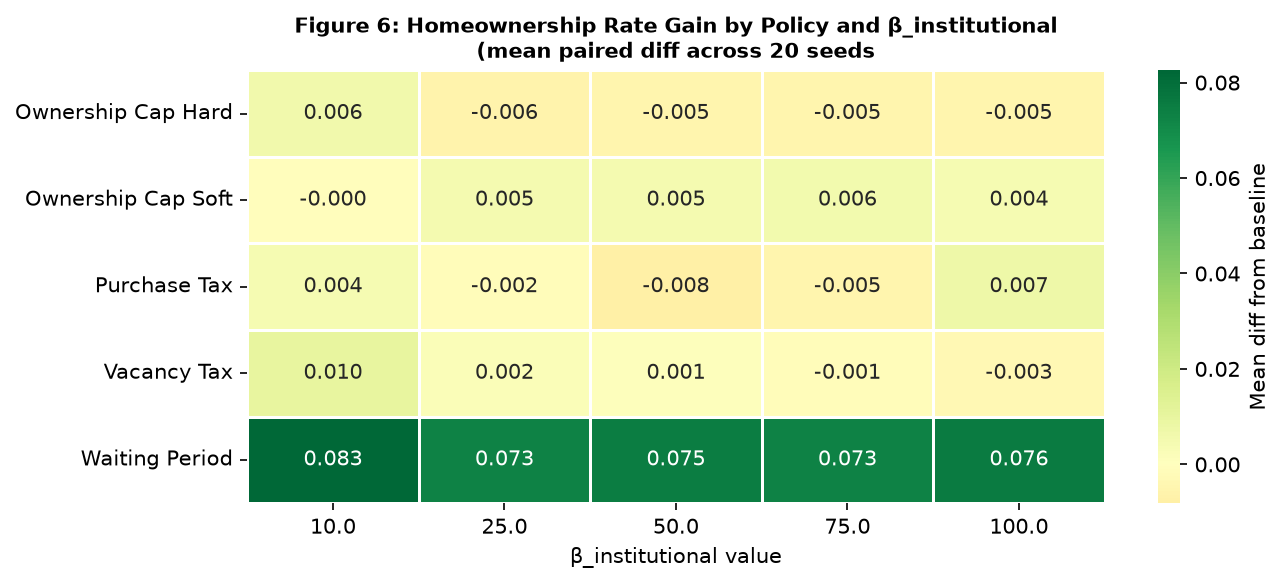
\includegraphics[width=1\linewidth]{figure6_sensitivity_heatmap.png}
    \caption*{Figure 5}
\end{figure}


Some parameters that could not be estimated through empirical means were approximated through sensitivity testing. In particular, $\beta_{\text{institutional}},$ which measures to what intensity investors react to yield signals, was tested across a range of plausible values and the policies. The heatmap in figure 5 reports the impact of each policy on the homeownership rate across the values of $\beta_{\text{institutional}}.$ \newline


\section{Discussion}
\subsection{Policy Effectiveness}
The results of the policy comparison reveal a consistent pattern: access restrictions are more effective than financial penalties with regards to first-time homeownership rate. Furthermore, among access restrictions, the waiting period dominates. \newline

The waiting period produces a mean paired difference of +3.3\% relative to baseline.  By preventing investors from bidding on newly listed houses for a set amount of periods, the waiting period gives first time buyers exclusive access to fresh listings during their most competitive period. Traditionally, investors, with access to increased capital and resources, outbid first time buyers and force them out of the market. The waiting period solves this problem by guaranteeing access to desired houses for first time buyers without exorbitant price inflation. The ownership cap, bot the hard and soft variant, also improve homeownership at rates of +1.6\% and +0.6\% respectively. \newline

However, the waiting period is the only policy that measurably improves rental vacancy and homeownership rate. Because the restriction slows investors without forcing them to sell their units,  existing rental stock is preserved while  new listings tilt towards owner-occupants. On the other hand, when applying the ownership caps, the rental supply may slow down at a rate faster than the renter population slows, causing vacancy to decrease. The net effect is a tighter rental market alongside higher homeownership, a realistic tradeoff. The waiting period mechanism avoids this tightening, as it still allows investors to purchase units, albeit with a delay.  \newline

All three financial penalties produce negligible or negative effects on homeownership rate. The vacancy tax produces negative effects on both homeownership and rental vacancy: the tax successfully incentivizes investors to fill their rental units, which in turn tightens the market. As overall transaction dynamics are disrupted, homeownership takes a slight hit. \newline

The consistent underperformance of the financial penalties in our simulation reflects the differences of how these policies act in the real world. Financial penalties function by decreasing investor expected yield. However, because investors have strong yield signals and access to a high amount of capital, the margin of purchase shifts only slightly. On the other hand, access restrictions outright prevent investors from placing bids on houses, which directly reduces investor competition rather than decreasing the probability. 

\subsection{Implications for US Policy}
The 21st Century ROAD to Housing Act prohibits investors from purchasing additional single-family homes, a policy that most closely resembles the soft ownership cap from our model. Our results suggest that this policy produces an improvement of homeownership, at the cost of tightening the rental market for people not ready to purchase homes yet. Policymakers should anticipate this side effect, and implement measures to protect rental supply, which we see through build-to-rent exemptions in this legislation. Other protections could be to increase upzoning, increasing housing production as a supply-side reform. \newline

The waiting period, which has been implemented at the local level in states like Oregon and New York, performs better than the ownership cap on both primary outcomes in the model. Unlike the cap, it does not require tracking of portfolio sizes, and our results suggests it achieves similar or better increases in homeownership without tightening rental supply. \newline

The poor performance of financial penalties suggests that price-based policies are insufficient to shift investor behavior in markets with a strong long-term yield. Atlanta's 2026 gross rental yield of 8.28\% provides a cushion against modest tax surcharges. Increased taxing rates and combinations of financial penalties may be necessary to meaningfully improve metrics, though we leave this for future work. \newline

\subsection{Limitations \& Future Work}

There are some limitations of the model that should be noted. Firstly, the model operates on a single, representative census tract rather than the full tract grid of Atlanta's metro area. This necessarily excluded geographic restrictions which prevent bidding on specific census tracts for institutional investors. Later models should incorporate a larger geographic region to model displacement effects. \newline

Second, confidence intervals are wide and the share of seeds moving in the same direction is not substantially above chance. The results should be treated as directional rather than precise values, and future work should increase run time and number of seeds for Monte Carlo simulations in order to create deterministic results.\newline

Third, policies were solely tested individually, when in reality many pieces of legislation propose combinations of the discusses policies. Future work should test distinct combinations of policies to reveal different effects. \newline

Fourth, microdata was not directly sampled from the PUMS dataset, which could be a future adaption. Rather, aggregate statistics were used to sample from a simplified distribution. Furthermore, certain parameters were gathered from literature not tuned to Atlanta, and should be tested with sensitivity analysis to see how a range of values impacts the core metrics. \newline

Finally, certain dynamics are difficult to model in code but could play a role in realistic responses to policy interventions. In particular, we are aware that investors may try to evade policies by artificially dividing into smaller portfolios that do not meet our definition of institutional investors. Our models classification of agents based on portfolio size fails to capture this dynamic, which may impact our results when translated to the real world. \newline








\section{Conclusion}
This paper develops and calibrated an agent-based model of the Atlanta, Georgia housing market to test the effectiveness of six institutional investor restriction policies across two outcome metrics: first-time homeownership rate and rental vacancy rate. Using empirical data from the ACS, HMDA, Zillow and Case-Shiller databases, the model is initialized to 2019 Atlanta conditions and run forward through Monte Carlo simulations across 40 seeds per scenario. \newline

The central finding is that access restrictions surpass financial penalties in increasing first-time homeownership, and that waiting period dominates all policies testing. At $3.3\%$ percentage points about baseline, the waiting period produces the largest homeownership improvement while loosing rental supply. The hard ownership cap gives a modest gain in homeownership while slightly constricting the rental market in doing so. Financial penalties (purchase tax, vacancy tax, progressive portfolio tax) have negligible or negative effects across all metrics, reflecting investors' low sensitivity to cost increases when long term yield is so high. \newline

These findings carry implications for the 21st Century ROAD to Housing Act of 2026. The legislation's ownership ban resembles our soft ownership cap, which our model predicts will improve homeownership but reduce rental supply. The build-to-rent exemptions included in the Act are a reasonable offset to this anticipated trade-off. More broadly, our results suggest that waiting period mechanisms, which give owner-occupiers first priority for desirable homes, achieves comparable or superior homeownership outcomes while preventing rental supply costs, and should be considered as an alternative to ownership bans. \newline

Several limitations hinder these conclusions. The single-tract structure prevents implementation of geographic restriction policies and fails to represent displacement dynamics. Confidence intervals are wide for individual policies, particularly financial penalties, and are not distinguishable from 0 in many seeds. Results should be interpreted as directional rather than precise. \newline

Future work should extend the model to the full Atlanta metro tract grid to capture displacement, incorporate direct PUMS microdata sampling, and test combinations of policies to see if they produce complementary effects. Longer simulations and higher seed counts would strengthen the precision of the Monte Carlo estimates. These extensions would overall allow the model to be a more representative tool to evaluate other policies, like the geographic restriction, or combinations of policies, like issuing multiple taxes, on their effectiveness in promoting homeownership nationwide. 


\section*{acknowledgments}

I would like thank my mentor, Arnold Yang, for his assistance throughout the project development and execution.


\bibliographystyle{IEEEtran}
\bibliography{references}

\appendix
\section{Model Equations}
This section specifies the full set of equations used, adapted from Axtell et al. (2014) and Baptista et al. (2016) with modifications to fit the Atlanta specific market. Greek letters refer to calibrated constants. 



\subsection{Household Wealth and Consumption}
 
\textbf{Equation 1 (Desired bank balance).} Household wealth  follows a log-normal relationship with income, estimated from Survey of Consumer Finances microdata:
$$
\ln(w) = \alpha + \beta \ln(y) + \varepsilon
$$
where $w$ is the desired bank balance, $y$ is income, and $\varepsilon$ is Gaussian noise.
 
\textbf{Equation 2 (Consumption).} Monthly consumption is a fraction of the gap between current bank balance $b$ and desired balance $w$:
$$
C = \max\big(\alpha(b - w),\ 0\big).
$$
\subsection{Buying, Selling, and Pricing}
 
\textbf{Equation 3 (Desired expenditure).} A household's desired purchase price scales with income and apprecation.
$$
p_{\text{desired}} = \frac{\alpha\, y\, \exp(\varepsilon)}{1 - \beta g}
$$
where $g$ is the expected monthly appreciation rate (Equation 4). For institutional investors, $y$ is replaced with available capital, and $\alpha$ is calibrated separately.
 
\textbf{Equation 4 (Price appreciation expectation).} Agents look at past home price indices to estimate the yearly annual appreciation. 
$$
g_t = \alpha \left( \frac{h_{t-1} + h_{t-2} + h_{t-3}}{h_{t-13} + h_{t-14} + h_{t-15}} - 1 \right)
$$
where $h_i$ is the house price index in month $i$.
 
\textbf{Equation 5 (Buy vs.\ rent decision).} Households compare the  cost of renting to the  cost of owning and apply a logistic function to make the choice:
$$
P(\text{buy}) = \sigma\Big(\beta \big[ r_Q(1+\tau) - 12(m - p g) \big]\Big)
$$
where $\sigma(x) = 1/(1+e^{-x})$, $r_Q$ is the annual rent for a house of quality $Q$, $\tau$ is a psychological preference for ownership , $m$ is the monthly mortgage payment, and $p$ is desired expenditure from Equation 3. 
 
\textbf{Equation 6 (Selling probability).} Homeowners sell at a probability that considers average tenure, interest rates and mortgage rate lock in effect: 
$$
P(\text{sell}) = \frac{1}{12} (\frac{1}{\text{tenure}}\Big[1 + \alpha(\bar{n}_h - n_h) + \beta(\bar{\imath} - i) + \gamma(i - i_{\text{mortgage}})\Big])
$$
where $n_h$ is houses per capita on the market, $i$ is the current mortgage interest rate, and $\gamma(i - i_{\text{mortgage}})$ reduces selling rate for higher mortgages.


\textbf{Equation 7 (Asking price).} Sellers set listings by comparing recent prices for similar quality houses in the area. 
$$
\ln p_s = \alpha + \ln(\bar{p}) - \beta \ln\big(\zeta(1+\bar{f})\big) + \varepsilon
$$
where $\bar{p}$ is the tract-level average sold price for comparable quality and $\bar{f}$ is average days-on-market. 
 
\textbf{Equation 8 (Price reduction).} Unsold listings face a chance of markdown each period:
$$
p_t = \begin{cases} p_{t-1}\big(1 - \exp(\varepsilon)\big), & \text{with probability } P_{\text{reduce}} \\ p_{t-1}, & \text{otherwise} \end{cases}
$$
 
\subsection{Investor Yield and Rental Pricing}
 
\textbf{Equation 9 (Expected yield, purchase decision).} Small landlord and institutional investor agents see if they should purchase by blending capital appreciation (long term profits) and rental yield (steady income)
$$
\Omega = \frac{p}{d}\big(\delta(g+\kappa) + (1-\delta)\bar{r}\big) - \frac{m}{d} - \text{policy cost}
$$
where $d$ is the down payment, $\kappa$ is the average gross rental yield, $\bar{r}$ is the current tract-level gross yield, and $\delta$ is the weight placed on capital gain versus rental income ($\delta = 0.3$ for small landlords, $\delta = 0.6$ for institutional investors). Financial penalties increase the policy cost term. 
 
\textbf{Equation 10 (Purchase probability).} The probability of proceeding with a purchase is:
$$
P_{\text{buy}} = \sigma(\beta \Omega)^{1/12}
$$
 $\beta_{\text{institutional}}$ is treated as uncertain and swept in the sensitivity analysis of Section~5. Hard policy restrictions set probability of buying at zero. 
 
\textbf{Equation 11 (Rental pricing).} Small landlords reprice with a certain probability (stickiness). Institutional investors instead price directly to market rate at every renewal with no stickiness.
$$
\ln q_{\text{small landlord}} = \alpha + \ln(\bar{r}) - \beta \ln\big(\zeta(1+\bar{f})\big) + \varepsilon, \quad \text{w.p. } p_{\text{reprice}}
$$

$$
q_{\text{institutional}} = \bar{r} \times (1 + \text{premium})
$$

 
\textbf{Equation 12 (Effective yield, sale decision).} Investors consider yield from current properties to see if they should sell.
$$
\Psi = \frac{p}{u}\big(\delta(g+\kappa) + (1-\delta)\bar{r}\big) - \frac{m}{u} - \text{policy cost}
$$
where $u = p - $ mortgage principal is current equity, bounded by 0. Vacancy tax and portfolio tax reduce yield, making it more likely to sell. 
 
\textbf{Equation 13 (Sale probability).}
$$
P_{\text{sell}} = 1 - \sigma(\beta \Psi)^{1/12}
$$
Hard enforcement caps set probability of selling at 1 (like forced divestiture). 
 
\subsection{Mortgages and Down Payments}
 
\textbf{Equation 14 (Owner-occupier mortgage approval).} The maximum loan amount is the minimum of two constraints:
$$
q = \min\left( \frac{b\chi}{1-\chi},\ y_d \nu \frac{1-(1+i_R)^{-N}}{i_R} \right)
$$
where $\chi$ is the maximum loan-to-value ratio (FHA: $\chi = 0.965$; conventional: $\chi = 0.80$), $y_d$ is disposable income net of essential consumption, $\nu$ is the maximum share of disposable income allocated to housing payments, and $i_R$, $N$ are the monthly mortgage rate and loan term. 
 
\textbf{Equation 15 (Investor mortgage underwriting).} Investor mortgages are subject to a debt-service coverage constraint.
$$
\Lambda < \frac{b}{1 - \dfrac{\bar{y}_r}{\xi\, i_{\text{BTL}}}}
$$
where $\bar{y}_r$ is the moving average gross annual rental yield on new tenancies, $\xi$ is the required interest coverage ratio, and $i_{\text{BTL}}$ is the investor mortgage rate.
 
\textbf{Equation 16 (Mortgage interest rate).} Rather than calculating interest rate within the model, we keep it constant and outside of the model (exogenous). 
 
\textbf{Equation 17 (Owner-occupier down payment).} Down payment is drawn from a two-part mixture reflecting a proportion of buyers who pay the minimum amount, and log-normal distribution above it, fit with HMDA data:
$$
d = \begin{cases} d_{\text{minimum}}, & \text{income rank} \le \text{income cutoff} \\ \max\big(d_{\text{minimum}},\ p \cdot F^{-1}(\cdot)\big), & \text{otherwise} \end{cases}
$$
where $F$ is a log-normal distribution fit only to people who paid above minimum, and the income cutoff is set to match the  loans who paid the minimum down payment.
 
\subsection{Market Clearing}
 
\textbf{Equations 18--20 (Double-auction clearing).} Both the ownership and rental markets clear by a multi-round double auction. Investor bids are matched to the offer with the highest expected yield they can afford,
\begin{equation}
E(y_q) = \frac{12\, r_q\, E(o_q)}{p}
\end{equation}
where expected occupancy $E(o_q)$ comes from typical US lease length (12 months).
\begin{equation}
E(o_q) = \frac{365}{365 + \bar{D}_q}
\end{equation}
Household (non-investor) bids are instead matched to the highest-quality affordable offer. When a house has multiple bids, the price is raised upward, and the winner is chosen randomly from people who can still afford the house. Bids that fail reenter the bidding pool for another round, and unmatched bids go back to renting and bid again next month. 
\end{document}